%Input preamble
\documentclass[11pt]{article}

% colors
\usepackage[table]{xcolor}
\definecolor{maroon}{RGB}{153,0,18}
\definecolor{lime}{RGB}{190,213,88}
\definecolor{sand}{RGB}{217,202,179}
\definecolor{fire}{RGB}{144,50,61}
\definecolor{brick}{RGB}{94,11,21}
\definecolor{olive}{RGB}{117,109,84}
\definecolor{lavpink}{RGB}{172,123,132}
\definecolor{darkpurp}{RGB}{49,10,49}
\definecolor{salmon}{RGB}{204,90,113}
\definecolor{mauve}{RGB}{94,73,85}
\definecolor{greyblue}{RGB}{125,132,145}
\definecolor{greypurp}{RGB}{68,56,80}
\definecolor{brightpurp}{RGB}{96,20,255}

% packages (please add in alphabetical order)
\usepackage{adjustbox}
\usepackage{amsfonts}
\usepackage{amsmath}
\usepackage{amssymb}
\usepackage{array}
\usepackage{bm}
\usepackage{booktabs}
\usepackage{caption}
\usepackage{epstopdf}
\usepackage{float}
\usepackage[margin=1in]{geometry}
\usepackage{graphicx}
\usepackage[colorlinks=true, linkcolor=brightpurp, citecolor=brightpurp, urlcolor=salmon]{hyperref}
\usepackage{lipsum}
\usepackage{longtable}
\usepackage{mathtools}
\usepackage{multirow}
\usepackage{natbib}
\usepackage{rotating}
\usepackage{setspace}
\usepackage{subcaption}
%\usepackage{threeparttable}
\usepackage{threeparttablex}
\usepackage{xr}
\usepackage[printwatermark]{xwatermark}


\newcolumntype{L}[1]{>{\raggedright\let\newline\\\arraybackslash\hspace{0pt}}m{#1}}
\newcolumntype{C}[1]{>{\centering\let\newline\\\arraybackslash\hspace{0pt}}m{#1}}
\newcolumntype{R}[1]{>{\raggedleft\let\newline\\\arraybackslash\hspace{0pt}}m{#1}}

% commands
\newcommand{\mr}{\multirow}
\newcommand{\mc}{\multicolumn}

%Other parameters
\newcommand{\noutcomes}{95}
\newcommand{\treatsubsabc}{$75\%$}
\newcommand{\treatsubscarec}{$74\%$}
\newcommand{\treatsubscaref}{$63\%$}

%Counts
%Males
\newcommand{\positivem}{$79\%$}
\newcommand{\positivesm}{$37\%$}

%Females
\newcommand{\positivef}{$73\%$}
\newcommand{\positivesf}{$35\%$}

%Counts, control substitution
%Males
\newcommand{\positivecsnm}{$58\%$}
\newcommand{\positivescsnm}{$25\%$}

\newcommand{\positivecsam}{$74\%$}
\newcommand{\positivescsam}{$38\%$}

%Females
%% no alternative
\newcommand{\positivecsnf}{$83\%$}
\newcommand{\positivescsnf}{$46\%$}

%% alternative
\newcommand{\positivecsaf}{$73\%$}
\newcommand{\positivescsaf}{$23\%$}

%Pooled

%Effects
%Males

%Females
\newcommand{\hsgradf}{$7$}
\newcommand{\yearsedf}{$1.2$}



%Pooled

%CBA
%IRR
%Males
\newcommand{\irrm}{$15\%$}
\newcommand{\irrsem}{$13\%$}

%Females
\newcommand{\irrf}{$10\%$}
\newcommand{\irrsef}{$12\%$}

%Pooled
\newcommand{\irrp}{$13\%$}
\newcommand{\irrsep}{$11\%$}

%BC
%Males
\newcommand{\bcm}{$7.88$}
\newcommand{\bcsem}{$8.06$}

%Females
\newcommand{\bcf}{$2.30$}
\newcommand{\bcsef}{$1.56$}

%Pooled
\newcommand{\bcp}{$4.35$}
\newcommand{\bcsep}{$2.57$}

%NPV streams
%Pooled
\newcommand{\parincomenpvp}{$\$115,026$}

\newcommand*\leftright[2]{%
  \leavevmode
  \rlap{#1}%
  \hspace{0.5\linewidth}%
  #2}

\newcommand{\orth}{\ensuremath{\perp\!\!\!\perp}}%
\newcommand{\indep}{\orth}%
\newcommand{\notorth}{\ensuremath{\perp\!\!\!\!\!\!\diagup\!\!\!\!\!\!\perp}}%
\newcommand{\notindep}{\notorth}

\externaldocument{abc_treatmenteffects_appendix}
\pagenumbering{roman}

\begin{document}

\begin{titlepage}
\newgeometry{top=.8in, bottom=.8in, left=.8in, right=.8in}

\title{\Large \textbf{Gender Differences in\\ the Benefits of an Influential Early Childhood Program}\thanks{This research was supported in part by grants from the Robert Wood Johnson Foundation's Policies for Action program, NICHD R37HD065072, the American Bar Foundation, the Buffett Early Childhood Fund, the Pritzker Children's Initiative, NICHD R01HD054702, NIA R01AG042390, and by the National Institute On Aging of the National Institutes of Health under Award Number P30AG024968. The views expressed in this paper are solely those of the authors and do not necessarily represent those of the funders or the official views of the National Institutes of Health. The authors wish to thank Frances Campbell, Craig and Sharon Ramey, Margaret Burchinal, Carrie Bynum, Elizabeth Gunn, and the staff of the Frank Porter Graham Child Development Institute at the University of North Carolina Chapel Hill for the use of data and source materials from the Carolina Abecedarian Project and the Carolina Approach to Responsive Education. They also assisted with information on the implementation of the studied interventions. Years of partnership and collaboration have made this work possible. We thank Ruby Zhang for excellent research assistance. Collaboration with Andr\'{e}s Hojman, Yu Kyung Koh, Sylvi Kuperman, Stefano Mosso, Rodrigo Pinto, Joshua Shea, and Jake Torcasso on related work has strengthened the analysis in this paper. For helpful comments on various versions of the paper, we thank the editor, three anonymous referees, St\'{e}phane Bonhomme, Fl\'{a}vio Cunha, Steven Durlauf, David Figlio, Marco Francesconi, Dana Goldman, Ganesh Karapakula, Sidharth Moktan, Rich Neimand, Tanya Rajan, Azeem Shaikh, Jeffrey Smith, Chris Taber, Matthew Tauzer, Ed Vytlacil, Jim Walker, and Matt Wiswall. We benefited from helpful comments received at the Leonard D. Schaeffer Center for Health Policy and Economics in December, 2016, and at the University of Wisconsin, February, 2017. For information on childcare in North Carolina, we thank Richard Clifford and Sue Russell. The set of codes to replicate the computations in this paper are posted in a repository. Interested parties can request to download all the files. The address of the repository is \url{https://github.com/jorgelgarcia/abccare-cba}. To replicate the results in this paper, contact any of the authors, who will put you in contact with the appropriate individuals to obtain access to restricted data. The Appendix for this paper is posted on \url{http://cehd.uchicago.edu/ABC_CARE}.}}

\author{
Jorge Luis Garc\'{i}a\\
Department of Economics\\
The University of Chicago \and
James J. Heckman \\
American Bar Foundation \\
Department of Economics\\
The University of Chicago \and
Anna L. Ziff \\
Center for the Economics of \\
Human Development \\
The University of Chicago}
\date{First Draft: January 5, 2016\\ This Draft: \today \\}

\maketitle
\thispagestyle{empty}
\restoregeometry
\end{titlepage}

\thispagestyle{empty}
\singlespacing
\begin{abstract}
\noindent This paper studies the life-cycle impacts of a high-quality, intensive, influential, and widely emulated early childhood program that started early in life (at 8 weeks of age) and had a randomized design. Upon the impracticality of analyzing the dozens of outcomes available to evaluate the program one at the time and the need to avoid cherry-picking outcomes with significant treatment effects, we propose parametric and non-parametric tests to aggregate and summarize treatment effects. We document that girls benefit more than boys. The source of this difference is a worst counterfactual to treatment for girls which results from baseline socio-economic disadvantage. \textbf{[Word count: 100 words.]}

\end{abstract}

\noindent \textbf{Keywords}: Gender differences, childcare, early childhood education, randomized trials, substitution bias \\
\noindent \textbf{JEL codes}: J13, I28, C93\\


\bigskip
\begin{tabular}{ll}
Jorge Luis Garc\'{i}a                                       & James J. Heckman \\
Department of Economics                                & Department of Economics \\
University of Chicago                                       & University of Chicago \\
1126 East 59th Street                                     & 1126 East 59th Street \\
Chicago, IL 60637                                           & Chicago, IL 60637 \\
Phone: 773-449-0744                                    & Phone: 773-702-0634  \\
Email: jorgelgarcia@uchicago.edu                       & Email: jjh@uchicago.edu \\
                                                                       & \\
Anna L. Ziff                                         &  \\
Center for the Economics of & \\
Human Development            & \\
University of Chicago                                        &  \\
1126 East 59th Street                       & \\
Chicago, IL 60637                                              &       \\
Phone: 734-277-7379                                    &  \\
Email: aziff@uchicago.edu                     &  \\

\end{tabular}

\clearpage

\vspace{3 em}
\noindent \textbf{[JJH: I need the web appendix---not printed.][This is printed now.]} \\

\noindent \textbf{[JJH: Before we spoke about low quality childcare harming boys. Now suddenly this has gone and replacing it wis high quality home environments for boys. Are we so sure?]} \\

\noindent \textbf{This does not contradict what we have before. Before we stated the finding as ``boys being harmed by low quality program.'' But there is much more to this. In general, girls are more disadvantaged than boys so it needs to be the case that they face a worst treatment counterfactual, whether they stay at home or go to an alternative preschool (Panel (b) of Figure 2).} \\

\noindent \textbf{When exploring within-girls and within-boys is when we are able to better understand the interpretation of the different parameters that we estimated. Boys who are more disadvantaged more often go to alternatives (Panel (d), Figure 2). For girls, the reverse is true (Panel (c) of Figure 2). Then, boys benefit more from treatment if compared than alternatives than if compared to staying at home (at home their environment is better, else they are more disadvantaged and also they face a low quality alternative) --- as we discussed in the previous version. Girls benefit more from alternatives because else they would face a relatively worst home environment --- which we also discussed in the previous version.} \\

\noindent \textbf{We perform tests to verify that the patterns in Figure 2 are statistically significant and all of the batteries of tests agree to this interpretation: average effects sizes (which are nuts but a referee seems to obsess about them), combining functions (of the two types that we discusses), and the new tests (Rosenbaum).}
\vspace{3 em}

\clearpage

\restoregeometry
\doublespacing


\setcounter{page}{0}
\pagenumbering{arabic}

\setlength\parindent{0pt}
\setlength{\parskip}{10pt}

\section{Introduction}
\label{sec:introduction}


This paper studies two influential early childhood programs offered as an educational form of childcare. The programs are the Carolina Abecedarian Project (ABC) and its almost identical sister program, the Carolina Approach to Responsive Education (CARE), both evaluated by the method of random assignment---henceforth ABC/CARE. While certain features and categories of outcomes of ABC/CARE have been thoroughly assessed, our paper is the first to aggregate and summarize all of the available outcomes to evaluate the program, including, for example, adulthood administrative criminal records.

ABC/CARE was conducted in Chapel Hill, North Carolina for a sample of children born between 1972 and 1980. It was one of the pioneer programs that focused intensively on child-led learning and is a template for many current and proposed early childhood programs.\footnote{Programs inspired by ABC/CARE have been (and are currently being) launched around the world. \citet{Sparling_2010_Highlights} and \citet{Ramey_Ramey_Lanzi_2014_Interventions} list numerous programs based on the ABC/CARE approach. The programs are: IHDP---eight different cities around the U.S. \citep{Spiker-etal_1997_Helping}; Early Head Start and Head Start in the U.S. \citep{Schneider_McDonald-eds_2007_Scale-Up_Vol-1}; John's Hopkins Cerebral Palsy Study in the U.S. \citep{Sparling_2010_Highlights}; Classroom Literacy Interventions and Outcomes (CLIO) study in the U.S. \citep{Sparling_2010_Highlights}; Massachusetts Family Child Care Study \citep{Collins_etal_2010_Massachusetts-Study}; Healthy Child Manitoba Evaluation \citep{Healthy_Child_Manitoba_2015_Starting-Early}; Abecedarian Approach within an Innovative Implementation Framework \citep{Jensen_Nielsen_2016_ABC-Programme-Pilot}; and Building a Bridge into Preschool in Remote Northern Territory Communities in Australia \citep{UMonash_Dataset_2015_URL}. Educare programs are also based on ABC/CARE \citep{Educare_2014_Research_Agenda,Yazejian_Bryant_2012_Educare}.} It started at 8 weeks of age and continued through age 5. Treatment and control children were followed through their mid 30s, with data collected on multiple dimensions of human development. As a result of this intensive data collection, there are over 100 outcomes that we could use to evaluate the program.

Given the difficulty of individually analyzing the hundreds of available outcomes to evaluate the program and the need to avoid cherry-picking outcomes with significant treatment effects, we propose parametric and non-parametric tests to aggregate and summarize treatment effects. Table~\ref{table:summary} previews our approach. Panel (a) displays our summaries for early-childhood outcomes (birth to age 5). We offer four treatment-control comparisons across these outcomes by gender: (i) the average effect size; (i) the percentage of outcomes for which there is a positive treatment effect; (iii) the percentage of outcomes for which there is a positive and significant ($\alpha=10\%$) effect; and (iv) the asymptotic approximation of the $p$-value resulting from a non-parametric comparison of the joint distribution of outcomes \citep{Rosenbaum_2005_Distribution_JRSS}. Panels (b) and (c) are analogous for school age (ages 6 to 18) and adulthood (21 to 35), respectively, and Panel (d) includes all of the outcomes in Panels (a) through (c).


\begin{table}[!htpb]
\begin{threeparttable}
\caption{Summary of Treatment-Control Comparisons by Gender} \label{table:summary}
\centering 
\begin{tabularx}{16.5cm}{XcX}
& 

\begin{tabular}{lcccc} 
\toprule
 & \mc{2}{c}{\textbf{(a) Childhood}}   & \mc{2}{c}{\textbf{(b) School Age}}  \\
 & Females & Males & Females & Males \\
 \cmidrule(lr){2-3}  \cmidrule(lr){4-5}
 Average Effect Size &      \textbf{    0.367} &    \textbf{    0.316} &     \textbf{    0.395} &     0.214 \\  
 \% $>0$ Treatment Effect &    \textbf{   95.833}  &     \textbf{   75.000}	&	 \textbf{  100.000} &   \textbf{  100.000}  \\  
 \% $>0$, Significant Treatment Effect&     \textbf{   62.500}  &   \textbf{   37.500} &    \textbf{   55.556} &     \textbf{   44.444} \\  
\citet{Rosenbaum_2005_Distribution_JRSS} $p$-value &     \textbf{0.086} &     \textbf{0.086} 	&       \textbf{0.022} &     0.147 \\  
 \midrule
 & \mc{2}{c}{\textbf{(c) Adulthood}}   & \mc{2}{c}{\textbf{(d) All}}  \\
 & Females & Males & Females & Males \\
  \cmidrule(lr){2-3}  \cmidrule(lr){4-5}
 Average Effect Size  &     \textbf{    0.298} &    \textbf{    0.399} &     \textbf{    0.348} &  \textbf{0.327} \\  
 \% $>0$ Treatment Effect  &    \textbf{   88.889} &    \textbf{   72.222} & \textbf{   94.118} &    \textbf{   78.431} \\  
 \% $>0$, Significant Treatment Effect &    \textbf{   50.000}  &    \textbf{   33.333}	&    \textbf{   56.863}&    \textbf{   37.255} \\  
\citet{Rosenbaum_2005_Distribution_JRSS} $p$-value &     \textbf{0.010} &     \textbf{0.086} 	&       \textbf{0.010} &     \textbf{0.086} \\  
\bottomrule
\end{tabular}


% This table displays summaries of treatment effects by age and gender. Each of the panels contains statistics calculated using outcomes measured at the indicated ages. Early childhood includes outcomes measured before age 6, school age includes outcomes measured between age 6 and 18, and adult includes outcomes measured after 18. All (panel d), is a combination of all the outcomes in panels a-c. The average effect size is calculated by averaging over the effect size of the outcomes in the age category. The effect sizes of the individual outcomes are calculated by dividing the coefficient by the standard deviation of the control group. The $p$-values are asymptotic following \citet{Rosenbaum_2005_Distribution_JRSS}. The null hypothesis is that the control and treatment distributions, within gender, are equal. A $p$-value less than 0.1 indicates that the distributions are significantly different.  & 
\end{tabularx}
\begin{tablenotes}
\footnotesize
\item \textbf{Note:} This table displays summaries of treatment effects by age and gender. Each of the panels contains statistics calculated using outcomes measured at the indicated ages. Early childhood includes outcomes measured before age 6, school age includes outcomes measured between age 6 and 18, and adult includes outcomes measured after 18. All (panel d), is a combination of all the outcomes in panels (a) to (c). The average effect size is calculated by averaging over the effect size of the outcomes in the age category. The effect sizes of the individual outcomes are calculated by dividing the coefficient by the standard deviation of the control group. The \citet{Rosenbaum_2005_Distribution_JRSS} $p$-value originates from a test where the null is a common joint distribution of the variables in each category. A $p$-value less than $0.10$ (bolded) indicates that the distributions are significantly different at the 10\% level. More details on our inference procedure are in Section~\ref{sec:parameters}.
\end{tablenotes}
\end{threeparttable}
\end{table}

The first finding in Table~\ref{table:summary} is that randomized assignment to ABC/CARE benefited both females and males across the life cycle. Across the life-cycle, the average effect size for females (males) is $0.381$ ($0.254)$, the percentage of positive treatment effects is $94\%$ ($78\%$), and the percentage of significant treatment effects at the $10\%$ level is $43\%$ ($22\%$). Standard inference could be provided for these three measures. Instead, we provide the $p$-value of a non-parametric test contrasting the joint distribution of the outcomes. The conclusion from these comparisons aligns with the conclusions from the other measures, even in magnitude if the size of the $p$-value is taken as a measure of magnitude \citep{Fisher_1935_Inference_JRSS}. A disadvantage of our summaries is the loss of perspective on the magnitudes of the effects, which we describe and discuss further below.\footnote{For example, assignment to treatment increased college graduation for males by 17 percentage points, with a standard error of 5 percentage points and where the college graduation rate for the control group is 12\%. For females, assignment to treatment increased high school graduation by 25 percentage points, with a standard error of 1 percentage point and where the high school graduation rate for the control group is 53\% points. These results are the basis of the forecasts in \citet{Garcia_Heckman_Leaf_etal_2017_Comp_CBA_Unpublished}: The authors document that education is actually the main intermediate input when forecasting benefits across the life cycle.}

The second finding in Table~\ref{table:summary} is that females benefit more than males. This holds across the life cycle and across all of the measures that we employ to summarize the treatment effects. To explain the gendered treatment effects, we document that control-group girls grew up in a less favorable environment if compared to control-group boys using baseline measures (e.g.,\ less father presence, lower maternal education and IQ). Girls in the control group who stayed at home ($23\%$ of the control-group girls), were taken care of in a disadvantaged environment. Girls who went to preschools other than ABC/CARE ($77\%$ of the control-group girls), likely went to the lowest quality preschools because their families were more resource constrained if compared to their boy counterparts. Thus, girls benefited more from treatment because they would have otherwise grown up in a relatively worst environment if compared to boys.\footnote{Documentation in \citet{Burchinal_etal_1989_CD_Daycare-Pre-K-Dev} shows that the quality of the available alternatives was of lower quality than the treatment offered through ABC/CARE. We supplement this documentation with historical records showing that even the alternatives that followed state and federal standards of the era, were of lower quality than ABC/CARE as measured by concrete measures such as staff-child ratios. We provide more detail on the quality of ABC/CARE and the alternative options in Section~\ref{sec:data} and Appendix~\ref{appendix:background}.}

Although there was no significant difference in the take-up of preschool alternatives between control-group parents of girls and control-group parents of boys, there is a subtle, important difference in the within-gender take-up of alternatives. Within girls, take-up of alternatives does not differ significantly by socio-economic disadvantage, although we show later that more disadvantaged control-group parents of girls select home care. Within boys, the relatively advantaged stayed at home more often and did not attend the relatively low-quality preschool alternatives available in the area at the time when ABC/CARE was implemented. These results are verified when we estimate parameters that explicitly account for control substitution. That is, when we compare treatment to alternative preschools and treatment to staying at home. These parameters are not identified by randomization into treatment and require the stronger assumptions that we discuss below. Boys benefit the most from ABC/CARE when compared to alternative preschools, given their relatively better home environment. Girls benefit the most from ABC/CARE when compared to home environments, given that those who stay at home are more disadvantaged. The difference in this benefit is less than the difference for boys, which is consistent with the stronger presence of selection for boys.

ABC/CARE greatly benefits children by providing an enriching environment to complement their home environments. This sounds a cautionary note for advocates of early childhood programs in any form: Quality matters and low-quality programs could cause harm. Dissecting the counterfactual brings our results to a modern context in which many children are enrolled in preschool, and in which low-quality is abundant for children from socio-economic disadvantaged backgrounds.\footnote{Approximately 60\% of preschool-age children regularly receive non-parental childcare \citep{FIFCFS_2009_Wellbeing_REPORT}. At age 4, the child care break down for disadvantaged children, which compose 13\% of all children in the US \citep{USCB_2014_CoverageReport}, was the following. Head Start: 29\%; Non-Head Start center-based: 26\%; relative care: 15\%; non-relative care: 5\%; parental care: 25\%. While the quality of Head Start centers and family day care arrangements is constant across poor and non-poor children, the quality of the rest of arrangements is considerably and consistently lower for poor children, when compared to non-poor children. This according to Early Childhood Environment and family Dat Care scaled \citep{FIFCFS_2009_Wellbeing_REPORT}.}

The rest of our analysis unfolds in the following way. Section~\ref{sec:data} describes the experimental data we analyze and its special features. It documents the quality level of the alternative childcare that a considerable proportion of the control-group subjects attended. Section~\ref{sec:parameters} defines the treatment effects we estimate and how we summarize them. Section~\ref{sec:treatment-effects} reports the treatment effects overall and by gender and establishes the existence of sharp gender differences for many categories of outcomes. Section~\ref{sec:gender-differences} discusses the sources of these differences. Section~\ref{sec:conclusion} concludes.
	

\section{Data}
\label{sec:data}
We analyze a combined sample of the two closely related programs, ABC and CARE. Table~\ref{tab:abc-care-characteristics} summarizes their characteristics. Both interventions were implemented by researchers at the Frank Porter Graham Center (FPG) at the University of North Carolina Chapel Hill, and targeted children from disadvantaged families in the Chapel Hill area. ABC had four cohorts born between 1972 and 1977, and CARE had two cohorts born between 1978 and 1980. Eligibility was determined on the basis of the High Risk Index (HRI) developed for ABC and adapted for CARE \citep{Campbell_Wasik_etal_2008_ECRQ}. Components of the HRI include father's presence, parental employment, and participation in welfare.\footnote{See Appendix~\ref{app:eligibility-pop} for the full list of the determinants of HRI \citep{Ramey_Smith_1977_AJMD, Wasik_Ramey_etal_1990_CD, Ramey_Campbell_1991_childreninpoverty}.} Based on these eligibility requirements, \citet{Garcia_Heckman_Leaf_etal_2017_Comp_CBA_Unpublished} calculate that 43\% of all African American children would be eligible now and that 19\% were eligible during the intervention.

Both interventions involved free, intensive center-based care for subjects in the treatment group starting at 8 weeks and continuing until age 5 before the children started kindergarten. Treatment-group subjects also received daily health screenings, diapers, and formula until 6 months. Control-group families received diapers and formula as well for the same period of time \citep{Wasik_Ramey_etal_1990_CD,Ramey_Campbell_1991_childreninpoverty}. Between ages 5 and 8, there was an additional component of treatment in which home visitors worked with children and their parents to tutor the children and to encourage families to be involved in their child's schooling. In CARE, all the subjects who received center-based care also received this school-age component. In ABC, treatment status of this component was randomized. We do not analyze this part of the treatment because previous work has found this component of the treatment to have no significant effects \citep{Campbell_Ramey_etal_2002_ADS,Campbell_Conti_etal_2014_EarlyChildhoodInvestments}.

\begin{table}[!htbp]
\centering
\caption{Overview of the ABC and CARE Programs}
\label{tab:abc-care-characteristics}
\begin{threeparttable}
	\begin{tabular}{l l}
	\toprule
Site & Chapel Hill, North Carolina \\
Cohorts & 4 (ABC), 2 (CARE) \\
$N$ & 58 treatment, 56 control (ABC) \\
	& 17 treatment, 23 control (CARE) \\
\midrule
Eligibility & HRI $>$ 11 \\
		& Biologically healthy \\
\midrule
Treatment years & 1972--1981 (ABC), 1977--1985 (CARE) \\
Treatment duration & 5 years \\
\midrule
Home visits 	& 2.5--2.7	per month (CARE)	\\
Center care	& 50	weeks per year \\
		 	& 30--45 hours per week  \\
Other treatment components & Formula until 6 months\\
					& Diapers until 6 months \\ 
					& Health check-ups \\
					& Medical care \\
					& Parenting instruction \\
					& Counseling \\
					& Transportation to center \\
Control-group incentives & Formula until 6 months \\
				& Diapers until 6 months 	\\
				& Health check-ups until 1 year (ABC, cohort 1) \\
\midrule
Adult-child ratio & 1:3--1:6 \\
Teacher requirements & High school through masters \\
				& Experience with kids \\
Specialists & Physician, nurse, social worker \\
\bottomrule
\end{tabular}



\begin{tablenotes}
\footnotesize
\item Note: Characteristics that do not specify ABC or CARE were present in both. Biologically healthy includes lack of serious illness, including mental retardation. HRI is the High Risk Index. This table is adapted from \citet{Elango_Hojman_etal_2016_Early-Edu}. \\
\item Sources: \citet{Ramey_Collier_etal_1976_CarolinaAbecedarianProject,Ramey_Smith_1977_AJMD,Ramey_etal_1985_Project-CARE_TiECSE,Wasik_Ramey_etal_1990_CD,Ramey_Campbell_1991_childreninpoverty}. 
\end{tablenotes}
\end{threeparttable}
\end{table}

The program focused on developing language, cognition, and social-emotional skills. During ABC and CARE, the \textit{Learning Games} curriculum was developed and refined \citep{Sparling_Lewis_1979_BOOKLearninggamesFirstThree}. Other curricula used in the program emphasized child-led learning of skills important for future learning \citep{Ramey_Smith_1977_AJMD, Wasik_Ramey_etal_1990_CD, Ramey_Campbell_1991_childreninpoverty}. The teachers and classroom aids were trained continuously throughout the intervention. Researchers and child development experts at FPG observed the classroom interactions and relayed detailed feedback to the instructors \citep{Ramey-etal_2012-ABC}.

These aspects of the program relate to structural quality rather than process quality, i.e., the daily experiences of the children \citep{Thomason_LaParo_2009_EED}. Aspects of structural quality, including low child-teacher ratios, small group sizes, and teacher education, are often associated with high process quality \citep{Phillipsen_etal_1997_ECRQ}. However, recent studies find that curricula and professional development are even more highly correlated with process quality. This is especially true if the curricula and professional development are informed by knowledge of child development \citep{Slot_etal_2015_Dutch_ECRQ}. Although measures of process quality (e.g., measures of teacher-child interactions) are not available for the ABC/CARE subjects, the curricula and professional development offerings were exceedingly intensive, especially compared to standards of that era \citep{Ramey-etal_2012-ABC}. \textbf{[JJH: discussion off mark] [JLG: Yes, to me this is some real ed school bs, but referee 4 asks us to put this information in her ``minor'' comments 1.]}

CARE included an additional arm of treatment. Besides the services in Table~\ref{tab:abc-care-characteristics}, those in the treatment group also received home visiting from birth to age 5. Home visiting consisted of biweekly visits focusing on parental problem-solving skills. To individually test this home-visiting component, there was a third randomized group ($N=23$) that received only the home visiting component, but not center-based care \citep{Wasik_Ramey_etal_1990_CD}. In light of previous analyses finding no effect of this component, we drop this last group from our analysis.\footnote{\citet{Campbell_Conti_etal_2014_EarlyChildhoodInvestments} test and do not reject the hypothesis of no treatment effects for this additional component of CARE.} These analyses justify merging the treatment groups of ABC and CARE, even though that of CARE received the additional home-visiting component \citep{ABCCARE_Dataset}. We henceforth analyze the samples as coming from a single ABC/CARE program. This combination is also seen in \citet{Burchinal_etal_2006_MSRCD_IV-Growth-Curve}.

Table~\ref{tab:abccare-baseline} compares pre-program variables between experimental and gender groups. The only significant difference is seen in the HRI score, which is 1.78 points lower for males than for females. This indicates that males were slightly less advantaged at baseline. However, after accounting for multiple hypotheses using the Holm test, the difference in HRI score is no longer significant \citep{holm1979simple}.\footnote{For a more detailed description of the sample's disadvantage, see Appendix~\ref{app:eligibility-pop}.}

\begin{table}[!htbp]
\centering
\caption{Baseline Differences, ABC/CARE}
\label{tab:abccare-baseline}
\begin{threeparttable}
	\begin{tabular}{l c c c c c c}
\toprule
\mc{1}{c}{Variable} & Female & Male & $ p $ -value & Control & Treatment & $ p $ -value \\
& Mean & Differential & & Mean & Differential & \\
\midrule
Mother's age &                19.72 &                 1.13 &                 0.15 &                20.52 &                -0.51 &                 0.51 \\
Mother works &                 0.23 &                 0.09 &                 0.28 &                 0.21 &                 0.11 &                 0.18 \\
Mother's IQ &                84.46 &                 1.33 &                 0.46 &                84.65 &                 0.98 &                 0.58 \\
Father at home &                 0.24 &                 0.04 &                 0.56 &                 0.29 &                -0.05 &                 0.51 \\
Number of siblings &                 0.59 &                 0.07 &                 0.67 &                 0.71 &                -0.18 &                 0.29 \\
HRI score &                21.57 &                -1.78 &                 0.06 &                21.39 &                -1.47 &                 0.13 \\
Apgar score, 1 min. &                 7.68 &                -0.07 &                 0.80 &                 7.60 &                 0.09 &                 0.76 \\
Apgar score, 5 min. &                 8.94 &                -0.20 &                 0.33 &                 8.87 &                -0.04 &                 0.83 \\
Birthweight &                 7.18 &                -0.20 &                 0.34 &                 7.17 &                -0.19 &                 0.38 \\
Gestational age &                39.85 &                -0.42 &                 0.27 &                39.87 &                -0.50 &                 0.19 \\
\bottomrule
\end{tabular}
% This file generated by: /scripts/abccare/treatment-effects/abccare-baseline.do

\begin{tablenotes}
\footnotesize
\item Note: The variables in this table are all measured at the baseline age, close to when the children were born. A larger HRI (High Risk Index) score indicates more disadvantage. Apgar, measured at 1 and 5 minutes after birth, is a test of the health condition of newborn babies. A score closer to 10 indicates a healthier condition \citep{Apgar_1966_APGAR-Scoring_PCNA}. Birthweight is in pounds and gestational age is in weeks.
\end{tablenotes}
\end{threeparttable}
\end{table}

\indent \textbf{[JJH: Use Hold Test! Casual!] [JLG: Holm test in display now.]}


\subsection{The Randomization Protocol and its Compromises} \label{section:randomization}

Randomization for ABC/CARE was conducted on child pairs matched on family background. Siblings and twins were jointly randomized into either treatment or control groups. For siblings, this occurred when two siblings were close enough in age such that both of them were eligible for the program. Pairing was based on the High Risk Index, as well as maternal education, maternal age, and gender of the subject.\footnote{We do not know the original pairs.} 

ABC collected an initial sample of 121 subjects. All providers of health care and social services (referral agencies) in the area of the ABC/CARE study were informed of the programs. They referred mothers whom they considered disadvantaged. Eligibility was corroborated before randomization. Encouragement from the referral agencies was such that most referred mothers attended and agreed to participate in the initial randomization. We characterize each missing observation in Appendix~\ref{appendix:randomization}. In Appendix~\ref{appendix:estimates}, we document that our estimates are robust when we adjust for missing data using standard weighting (matching) methods described in Appendix~\ref{app:method_partialobs}. Twenty-two subjects in ABC did not stay in the program through age 5. The number of dropouts is evenly balanced across treatments and controls. Dropout was primarily related to the health of the child and the mobility of families rather than any dissatisfaction with the program. The 22 dropouts include four children who died, four children who left the study because their parents moved, and two children who were diagnosed as developmentally delayed. Details are in Table~\ref{table:abccompromises}. Everyone offered the program was randomized to either treatment or control. All eligible families agreed to participate. Dropping out occurs \emph{after} randomization and is balanced across treatment groups. We conduct the same analysis for the CARE sample, although there were far fewer dropouts and no compromised randomization.\footnote{The modest sample size, especially after dividing the sample by male and female, is unavoidable. No datasets have the experimental design and longitudinal data collection of ABC/CARE with a large sample. Future researchers should repeat these analyses in other, larger studies (e.g., the Infant Health and Development Program) as the subjects continue to age.} 

\subsection{Control Group Substitution}

In ABC/CARE, many control-group subjects (but no treatment-group subjects) attended alternative center-based care.\footnote{See \cite{Heckman_Hohmann_etal_2000_QJE} on the issue of substitution bias in social experiments.} The figure is \treatsubsabc\ for ABC and \treatsubscarec\ for CARE. This information is detailed in a survey administered to ABC/CARE families asking about the childcare arrangements made during each month between birth and age 5. Home care includes parental care, but also care of a relative, neighbor, or friend. The survey also captured specifics, such as the name of the center-based institutions, allowing for a more detailed understanding of the care environments.

\begin{sidewaysfigure}[!htbp]
\centering
\caption{Control Substitution Characteristics, ABC/CARE Control Group}\label{fig:control-sub}
\begin{subfigure}[h]{0.49\textwidth}
	\centering
	\caption{Cumulative Enrollment} \label{fig:treatsubcare}
	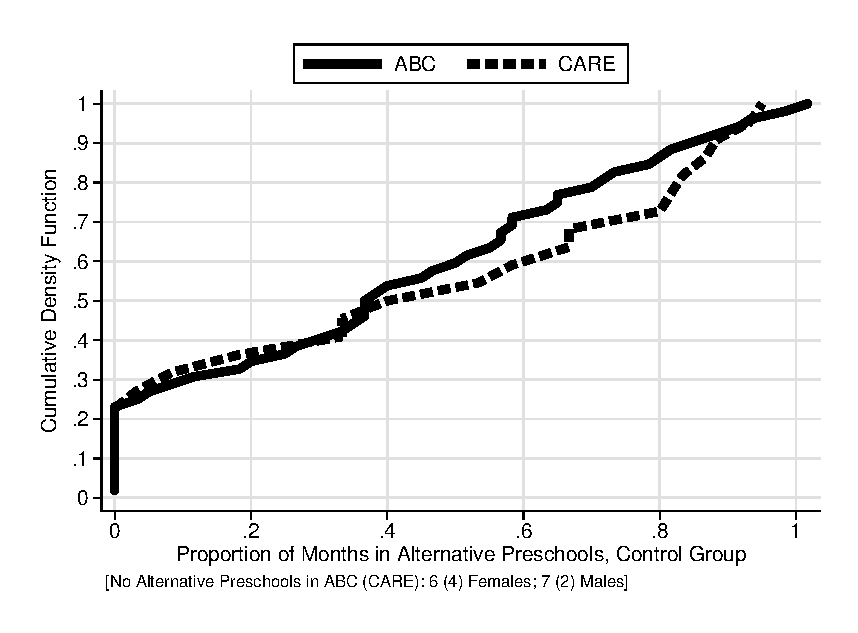
\includegraphics[width=\textwidth]{output/abccare_controlcontamination.eps}
\end{subfigure}
\begin{subfigure}[h]{0.49\textwidth}
	\centering
	\caption{Enrollment Dynamics} \label{fig:proportion-alt-pre}
	\includegraphics[width=\textwidth]{output/abccare_Vprobs.eps}
\end{subfigure}%
\footnotesize \justify
Note: Panel (a) displays the cumulative distribution function of enrollment in alternatives. Panel (b) displays the fraction of ABC/CARE control-group children enrolled in alternatives, conditional on being enrolled in the previous age (at least one month).\\
\end{sidewaysfigure}

Figure~\ref{fig:treatsubcare} shows the cumulative distribution of the proportion of time in the first five years that control subjects were enrolled in alternatives. Figure~\ref{fig:proportion-alt-pre} shows the dynamics of enrollment. Those who enroll generally stay enrolled. As control-group children aged, they were more likely to enter childcare (see Figure~\ref{fig:control-sub_a} in Appendix~\ref{app:control-subbb}).

Children in the control group enrolled in alternative early childcare programs are less economically disadvantaged at baseline compared to children who stay at home. Disadvantage is measured by maternal education, maternal IQ, Apgar scores, and the High Risk Index defining ABC/CARE eligibility. Children who attend low-quality alternative care have fewer siblings. On average, they are children of mothers who are more likely to be working at baseline (statistically significant at 10\%). Parents of girls are much more likely to use alternative center childcare if assigned to the control group. Table~\ref{table:controlsubscharacteristics} tests differences across these variables between children in the control group who attended and who did not attend alternative childcare. The only significant difference in observed characteristics is whether the mother works. For children attending alternative care, the mother is more likely to work. This is especially the case for female subjects. For male subjects, the labor supply of the mothers is statistically the same with 14\% of the mothers working for boys who stay at home. This is consistent with a higher percentage of fathers being present when the subject is male.

While most of the alternative childcare centers received federal subsidies and were subject to the federal regulations of the era, they were relatively low-quality compared to ABC/CARE \citep{Burchinal_etal_1989_CD_Daycare-Pre-K-Dev}. In terms of child-staff ratios, ABC/CARE far exceeded the highest state and federal standards compared to the alternatives.\footnote{Appendix~\ref{appendix:tetanus} shows this and discusses the federal standards of that day \citep{Department-of-Health_1968_DayCareRequirements,NCGA_1971_House-Bill-100,Ramey-et-al_1977_Intro-to-ABC,Ramey_Campbell_1979_SR,Ramey_McGinness_etal_1982_Abecedarianapproach,Burchinal_Campbell_etal_1997_CD}} We do not have complete information on the quality of the home care to be able to precisely analyze the environments of those who stayed at home. 

When we compare ABC/CARE treatment to these alternatives, ABC/CARE has substantial treatment effects. Further, as we argue below, parents perceived that ABC/CARE was superior to the alternatives. The access of control-group children to alternative programs creates both a problem of substitution bias \citep{Heckman_1992_randomization,Heckman_Hohmann_etal_2000_QJE, Kline_Walters_2016_QJE} and an opportunity to learn about the benefits or harms of low quality childcare arrangements. With the heterogeneous experiences of the control-group subjects, we can compare the effect of an enriched treatment against home and low-quality center environments separately.

\subsection{Data Collection}

Measures of cognitive, social-emotional, and parenting skills were collected during the intervention or while the subjects were in school.\footnote{Time use data are not available.} The researchers collected information on the subjects' academic performance including grade retention and special education. The adult surveys (at ages 21 and 30) cover items related to employment, post-secondary education, health, criminal activity, and family structure. When the subjects were in their mid 30s, the researchers collected administrative crime data and data from a full medical survey. Appendix~\ref{appendix:results} more completely describes the data that we use.




\section{Parameters of Interest}
\label{sec:parameters}
Random assignment to treatment does not guarantee that conventional treatment effect estimators answer policy-relevant questions. In this paper, we define and estimate three parameters that address different policy questions.

Let $W=1$ indicate that the parents referred to the program participate in the randomization protocol. $W=0$ indicates otherwise. $R$ indicates randomization into the treatment group ($R = 1$) or to the control group ($R = 0$). $D$ indicates attending the program, i.e., $D = R$ implies compliance with the initial randomization protocol.

Individuals are eligible to participate in the program if baseline background variables $\bm{B}\in\mathcal{B}_0$. $\mathcal{B}_0$ is the set of scores on the risk index that determines program eligibility. Because all of the eligible people given the option to participate choose to do so $(W=1\text{, and } D=R)$, we can safely interpret the treatment effects generated by the experiment as average treatment effects for the population for which $\bm{B}\in\mathcal{B}_0$ and not just treatment effects for the treated.

Let $\bm{Y}^1_a$ be the outcome vector at age $a$ for the treated. $\bm{Y}^0_a$ is the age-$a$ outcome vector for the controls. In principle, life-cycle outcomes for the treated and controls can depend on the exposures to various alternative preschools at each age. It would be desirable to estimate treatment effects for each possible exposure but our samples are too small to make credible estimates for very detailed levels of exposure. All treatment-group children have the same exposure to the ABC/CARE treatment and no exposure to alternative center-based care. 

We simplify the analysis of the controls by creating two categories. ``$H$'' indicates that the control-group child is in home care throughout the entire length of the program. ``$C$'' indicates that a control-group child is in alternative center childcare for any amount of time.\footnote{This assumption is consistent with Figure~\ref{fig:proportion-alt-pre}. Once parents decide to enroll their children in alternative childcare arrangements, the children stay enrolled up to age 5.} We test the sensitivity of our estimates to the choice of different categorizations in our empirical analysis in Appendix~\ref{appendix:vsensitivity-controlsub}.

We thus compress a complex reality into two counterfactual outcome states at age $a$ for control-group subjects:
\begin{align*}
\bm{Y}_{a,H}^0 \quad &: \quad \textbf{ Subject received home care exclusively} \\
\bm{Y}_{a,C}^0 \quad &: \quad \textbf{ Subject received some alternative childcare}.
\end{align*}

We define $V$ as a dummy variable indicating participation by control-group children in an alternative childcare. $V=0$ denotes staying at home. The outcome when a child is in control status is
\begin{equation}
\bm{Y}^0_a : = \left( 1 - V \right) \bm{Y}^0_{a,H} + \left( V \right) \bm{Y}^0_{a,C}. \label{eq:meandiff}
\end{equation}

One parameter of interest addresses the question: what is the effect of the program as implemented? This is the effect of the program compared to the next best alternative as perceived by the parents (or the relevant decision maker) and is defined by
\begin{equation}\label{eq:effect}
\bm{\Delta}_a := \mathbb{E} \left[ \bm{Y}^1_a -  \bm{Y}^0_a | W =1 \right] = \mathbb{E} \left[\bm{Y}^1_a - \bm{Y}^0_a | \bm{B} \in \mathcal{B}_0 \right],
\end{equation}
where the second equality follows because everyone who was eligible elected to participate in the program. For the sample of eligible people, this parameter addresses the effectiveness of the program relative to the quality of all alternatives available when the program was implemented, including staying at home. It is the parameter intended to be estimated by Local Average Treatment Effects (LATE; \citealp{Imbens_Angrist_1994_Econometrica}).

It is fruitful to assess the effectiveness of the program with respect to a counterfactual world in which the child stays at home full time. The associated causal parameter for those who would choose to keep the child at home is:
\begin{equation}\label{eq:influenza}
\bm{\Delta}_a \left(V = 0 \right) : =   \mathbb{E} \left[ \bm{Y}^1_a - \bm{Y}^0_a | V = 0, W = 1 \right] := \mathbb{E} \left[\bm{Y}^1_{a} - \bm{Y}^0_{a,H} | V = 0, \bm{B} \in \mathcal{B}_0 \right].\footnote{Appendix~\ref{appendix:vsensitivity-controlsub} displays results with alternative definitions of $V$ (i.e., different thresholds define if a child attended alternative childcare). The results are robust to the various definitions. What matters is whether any out-of-home child care is being used ($V>0$), and not the specific value of $V$.}
\end{equation}
It is also useful to assess the average effectiveness of a program relative to attendance in an alternative childcare center for those who would choose an alternative:
\begin{equation}\label{eq:smallpox}
\bm{\Delta}_a \left( V =1 \right) : =   \mathbb{E} \left[ \bm{Y}^1_a - \bm{Y}^0_a | V = 1, W = 1 \right] := \mathbb{E} \left[\bm{Y}^1_a - \bm{Y}^0_{a,C} | V = 1, \bm{B} \in \mathcal{B}_0 \right].
\end{equation}

Random assignment to treatment does not directly identify \eqref{eq:influenza} or \eqref{eq:smallpox}. Econometric methods are required to identify these parameters. We primarily rely on matching to control for selection into home or low-quality childcare by the control group. Our procedure assumes that the observed characteristics are sufficient to describe the selection into alternative center-based arrangements. We report results from alternative strategies, including instrumental variables and control functions, in Appendix~\ref{appendix:amethodology}. The results from these alternative strategies are consistent with our main results. We characterize the determinants of choices and our strategy for controlling for selection into home care (``$H$'') and alternative center-based care (``$C$'') when we discuss the empirical results in Section~\ref{sec:treatment-effects}.

\subsection{Summarizing Multiple Treatment Effects}\label{sec:combining-functions}

ABC/CARE has rich longitudinal data on multiple outcomes over multiple periods of the life cycle. Summarizing these effects in an interpretable way is challenging.\footnote{Appendix~\ref{appendix:results} presents step-down $p$-values for the blocks of outcomes that are used in the cost-benefit analysis of \citet{Garcia_Heckman_Leaf_etal_2017_Comp_CBA_Unpublished}. We follow the algorithm in \citet{Romano_Wolf_2016_pval_SaPL}.} Simpler, more digestible summary measures are useful for understanding our main findings. To construct these, we use combining functions that count the proportion of treatment effects that are positive by different categories of outcomes. 

In a companion paper \citep{Garcia_Heckman_Leaf_etal_2017_Comp_CBA_Unpublished}, we monetize outcomes and estimate rates of return and cost/benefit rates. This requires making an additional layer of assumptions to extrapolate lifetime benefits, which we avoid making in this paper. This cost/benefit analysis gives a weighted summary of the treatment effects, weighing by cost or benefit of the effect to society. The method described below does not weigh the individual effects by this or any other measure of ``importance.''

The combining functions provide us with an intuitive, digestible statistic. Despite being informative, the combining functions are admittedly arbitrary as an statistic such as are arbitrary, unweighted averages of treatment effects. We complement the tests arising from these functions with a non-parametric test on the joint distribution of outcomes grouped by categories developed by .

\noindent \textbf{Combining Functions.} Consider a block of $N_l$ outcomes indexed by set $Q_l = \{1,\dots,N_l\}$. Let $j \in Q_l$ be a particular outcome within block $l$. Associated with it is a mean treatment effect
\begin{equation}
\Delta_{j,a} : = \mathbb{E} \left[ Y^1_{j,a} - Y^0_{j,a} | \bm{B} \in \mathcal{B}_0 \right], j \in Q_l.
\end{equation}

We assume that outcomes can be ordered so that $\Delta_{j,a} >0$ is beneficial.\footnote{All but 5\% of the outcomes we study can be ranked in this fashion. See Appendix~\ref{appendix:results} for a discussion.} We summarize the estimated effects of the program on outcomes within the block by the count of positive impacts within block $l$:
\begin{equation}
C_l = \sum^{N_l}_{j=1} 1 (\hat{\Delta}_{j,a} >0).
\end{equation}
The proportion of beneficial outcomes in block $l$ is $C_l / N_l$.\footnote{In our empirical application we consider all the outcomes as a block, and then different blocks grouped according to common categories---e.g., skills, health, crime.}

Let $\mathcal{L}$ be the set of blocks. Under the null hypothesis of no treatment effects for all $j \in Q_l, l \in \mathcal{L}$, and assuming the validity of asymptotic approximations, $C_l / N_l$ should be centered around $\frac{1}{2}$. We bootstrap to obtain $p$-values for the null for each block and over all blocks. This procedure accounts for dependence in unobservables across outcomes. It also accounts for model pretesting. Bootstrapping allows us to account for dependence across outcomes (within blocks) in a general way. We adjust for pretesting by estimating a series of alternative models and computing the standard errors that account for doing so.

We also count the beneficial treatment effects that are statistically significant in the sets of outcomes across each of the groups indexed by the set $Q_l$. Using a 10\% significance level, on average 10\% of all outcomes should be ``significant'' at the 10\% level even if there is no treatment effect of the program. We provide evidence against both null hypotheses.\footnote{In this case, we perform a ``double bootstrap'' procedure to first determine significant treatment effects at $10\%$ level and then calculate the standard error of the count.} Combining counts across all blocks enables us to avoid (i) arbitrarily picking outcomes that have statistically significant effects---``cherry picking''; or (ii) arbitrarily selecting blocks of outcomes to correct the $p$-values when accounting for multiple hypothesis testing.\footnote{We present $p$-values for these hypotheses and a number of combining functions by outcome category in Appendix~\ref{appendix:results}.}$^{\text{,}}$\footnote{In Appendix~\ref{appendix:results} we present yet another alternative. We calculate a ``latent'' outcome out of the set of outcomes within a block and perform inference on this latent outcome. This analysis also points to beneficial effects of the program.} 

\section{Estimates and Tests}
\label{sec:treatment-effects}
In this paper, we focus on testing treatment effects within categories of outcomes or across all available outcomes. This is a powerful, comprehensive tool that allows us to summarize the impact of ABC/CARE and avoid problems such a cherry-picking statistically significant results. It has the downside of obscuring the interpretation of the magnitudes of the treatment effects in each of the outcomes of interest. To be as inclusive as possible, we categorize our outcomes and obtain a principal component per category. This principal component is a ``latent'' variable describing each category for which we can calculate treatment effects.

\begin{table}[!htpb]
\begin{threeparttable}
\caption{Combining Functions and Non-Parametric, Exact Tests} \label{table:massiveall}
\centering
\begin{tabular}{l c c c c}
\toprule
 & Average & \% $ >0 $ & \% $ >0 $ , Significant & \citet{Rosenbaum_2005_Distribution_JRSS} \\
 & Effect Size & Treatment Effect & Treatment Effect & $ p $ -value \\
\midrule
\textbf{IQ} & & & & \\
\quad Females &  \textbf{    0.796} & \textbf{  100.000} & \textbf{   57.143} & .046 \\
\quad Males &  \textbf{    0.981} & \textbf{  100.000} & \textbf{   85.714} & .045 \\
\midrule
\textbf{Achievement} & & & & \\
\quad Females &  \textbf{    0.623} & \textbf{  100.000} & \textbf{   40.000} & .046 \\
\quad Males &      0.253 & \textbf{  100.000} &    60.000 & .086 \\
\midrule
\textbf{Social-emotional} & & & & \\
\quad Females &  \textbf{    0.422} & \textbf{   85.714} & \textbf{   57.143} & .235 \\
\quad Males &      0.112 & \textbf{   71.429} & \textbf{   21.429} & .147 \\
\midrule
\textbf{Parental Income} & & & & \\
\quad Females &  \textbf{   -0.081} & \textbf{   80.000} & \textbf{   60.000} & .086 \\
\quad Males &      0.673 & \textbf{  100.000} &    60.000 & .001 \\
\midrule
\textbf{Parenting} & & & & \\
\quad Females &     -0.045 & \textbf{   80.000} & \textbf{    0.000} & .602 \\
\quad Males &      0.173 & \textbf{  100.000} & \textbf{    0.000} & .147 \\
\midrule
\textbf{Education} & & & & \\
\quad Females &  \textbf{    0.239} & \textbf{   83.333} & \textbf{   33.333} & 0 \\
\quad Males &      0.404 & \textbf{   66.667} & \textbf{   16.667} & .235 \\
\midrule
\textbf{Employment} & & & & \\
\quad Females &      0.013 & \textbf{  100.000} &     0.000 & .151 \\
\quad Males &     -0.032 & \textbf{  100.000} & \textbf{  100.000} & .022 \\
\midrule
\textbf{Crime} & & & & \\
\quad Females &      0.458 & \textbf{  100.000} & \textbf{   50.000} & .715 \\
\quad Males &     -0.382 &    33.333 &     0.000 & .812 \\
\midrule
\textbf{Risky Behavior} & & & & \\
\quad Females &      0.474 & \textbf{   66.667} & \textbf{   33.333} & .469 \\
\quad Males &      0.133 & \textbf{   25.000} & \textbf{   25.000} & .086 \\
\midrule
\textbf{Health} & & & & \\
\quad Females &      0.067 & \textbf{   73.333} & \textbf{   40.000} & .046 \\
\quad Males &      0.168 & \textbf{   53.333} & \textbf{    0.000} & 0 \\
\midrule
\bottomrule
\end{tabular}
% This file generated by: /scripts/abccare/genderdifferences/abccare-gdiff-raw-rosenbaum-table.do
 
\begin{tablenotes}
\footnotesize
\item \textbf{Note:} This table displays summaries of treatment effects by outcome category and gender. Each of the panels contains statistics calculated using outcomes grouped by category. The average effect size is calculated by averaging over the effect size of the outcomes in the outcome category. The effect sizes of the individual outcomes are calculated by dividing the coefficient by the standard deviation of the control group.  The \citet{Rosenbaum_2005_Distribution_JRSS} $p$-value originates from a test where the null is a common joint distribution of the variables in each category. Statistics significant at the $0.10$ level are bolded.
\end{tablenotes}
\end{threeparttable}
\end{table}

We consider the outcomes reported in Appendix~\ref{appendix:gdiff-tes}. In Table~\ref{table:summary}, we classify these outcomes by age to preview our results, aggregating outcomes within ages and across categories. In Table~\ref{table:massiveall}, we aggregate across ages and within categories. The benefits of random assignment to treatment are noticeable for both males and females. The benefits appear across the life cycle and across multiple outcomes. Participants of ABC/CARE benefit in terms of skills, both cognitive and socio-emotional. They also benefit in terms of achievement tests, which help measure both cognitive and non-cognitive skills \citep{Almlund_Duckworth_etal_2011_ecoval}.

[ADD ADDITIONAL DESCRIPTION ONCE TABLE IS DONE]

ABC/CARE had childcare, and thus facilitated maternal employment and education. This facilitated maternal employment and education. The program has a sizable effect on mother labor, which aggregates parental labor income and employment across the life cycle.\footnote{In most households, parental income and maternal income are the same: 75\% of children in the sample grew up in a household with a single mother.} This intergenerational effect is not only present in terms of parental income. It is also present in parenting, which aggregates HOME scores qualifying the relationship between the children and their mothers between ages 0 and 8.

In outcomes like education, employment, crime, risky behavior (which includes, for example, drug use) there is also a sizable effect. In our companion paper, \citet{Garcia_Heckman_Leaf_etal_2017_Comp_CBA_Unpublished}, we document that these effects translate into a benefit/cost ratio of $7.3$. This calculation accounts for the costs of implementing the program, including the welfare loss generated by taxing society in order to fund the program.

Consistent with the results in Table~\ref{table:summary}, the results in Table~\ref{table:massiveall} show that females benefit more from treatment if compared to males. In 7 out of the 10 categories that we consider, the within-category average effect size is larger for females. In 9 out of 10 categories, the proportion of positive effects is at least as large for males if compared to females. The same is true for the proportion of positive and significant effects, at the 10\% level. The comparison based on the \citet{Rosenbaum_2005_Distribution_JRSS} $p$-values is not as clear, which is one of the reasons why this difference deserves further assessment. We do so next.




\section{Explaining Gender Differences}
\label{sec:gender-differences}
This section discusses the factors generating gender differences. A major determinant is the choice of the alternative child care arrangements.
Estimated treatment effects are very similar across genders comparing treatment to staying at home full time. Males benefit much more from treatment relative to low quality childcare compared to their benefits from treatment relative to staying at home. This result is consistent with previous research that shows (i) substantial gender differences resulting from attending low quality childcare \citep{Kottelenberg-Lehrer_2014_Gender-Effects,Baker_Gruber_Milligan_2015_Noncog_Defects}; and (ii) that females are less sensitive to more stressful, low quality environments (see, e.g., \citealp{golding2016psychology,Autor-etal_2015_Family-Disadvantage}).

Table~\ref{tab:proportion-table-ranksign} shows the proportion of outcomes, by outcome category, for which the males exceed the females. Here, we further divide the control group into the alternatives used and both the treatment and control groups by father present, a potentially important moderator. Recall, we condition on baseline variables to control for selection into childcare for controls.\footnote{See Appendix~\ref{} for a sensitivity study using other methods. They produce the same estimates, but are less precisely estimated.} Figure~\ref{fig:proportion-altpre} shows the proportions partitioned by alternative childcare setting. The males who stay at home do better than the females in cognitive and parenting measures, employment, and across all outcomes. Unlike the males who attend lower quality alternative childcare, the males who stay at home have similar crime outcomes as the females. Given the important negative effects of male criminal activity, this finding highlights the magnitude of harm caused by low-quality alternative preschools for the males. 

\begin{figure}[H]
\centering
\caption{Proportion of Outcomes Males $>$ Females, by Outcome Category, Partitioning by Alternative Childcare Setting}
\label{fig:proportion-altpre}
	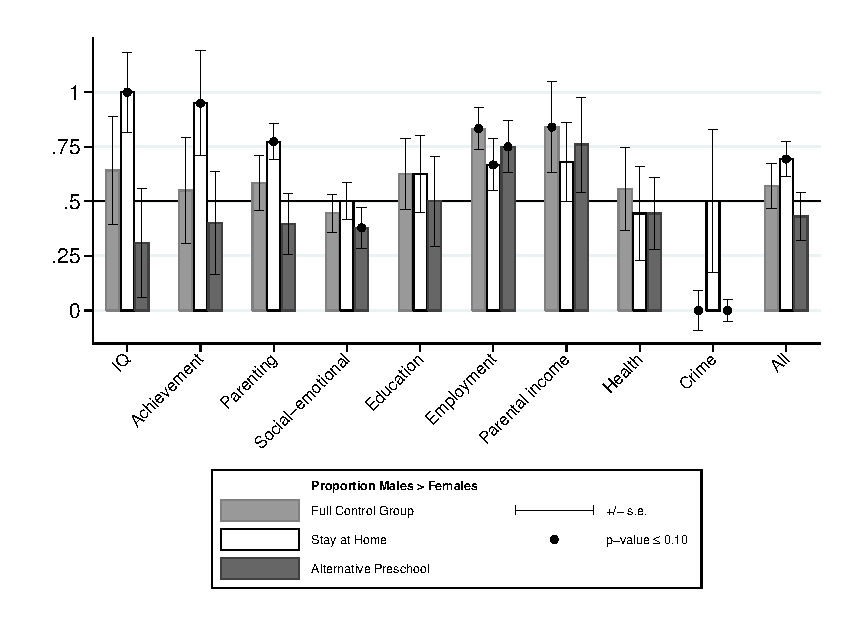
\includegraphics[width=\textwidth]{output/gendergaps-control-moderated-altpre}
\footnotesize \justify
Note: These plots show the proportion of outcomes, by outcome category, for which the males' mean is larger than the females' mean. The standard errors and the $p$-values are computed using 100 bootstraps. The $p$-values are one-sided and test the null hypothesis that the proportion of outcomes is greater than $\frac{1}{2}$ The crime outcomes are all coded so that a higher value indicates more criminal activity. All other outcome categories have higher values corresponding to socially desirable outcomes.
\end{figure}

In Appendix~\ref{}, we report estimates by whether or not the father is present (Figure~\ref{fig:proportion-fhome}). Few clear-cut patterns emerge. Father's presence interacted with treatment favors males for IQ, parenting, and health measures. Males in the control group do better when the father is absent in education and employment. This suggests that treatment complements the home environment for males more than for females.

\begin{figure}[!htbp]
\textbf{[JJH: Move to appendix.]}
\centering
\caption{Proportion of Outcomes Males $>$ Females, by Outcome Category, Partitioning by Whether or Not the Father is Present}
\label{fig:proportion-fhome}
\begin{subfigure}[h]{0.7\textwidth}
	\centering
	\caption{Control Group}
	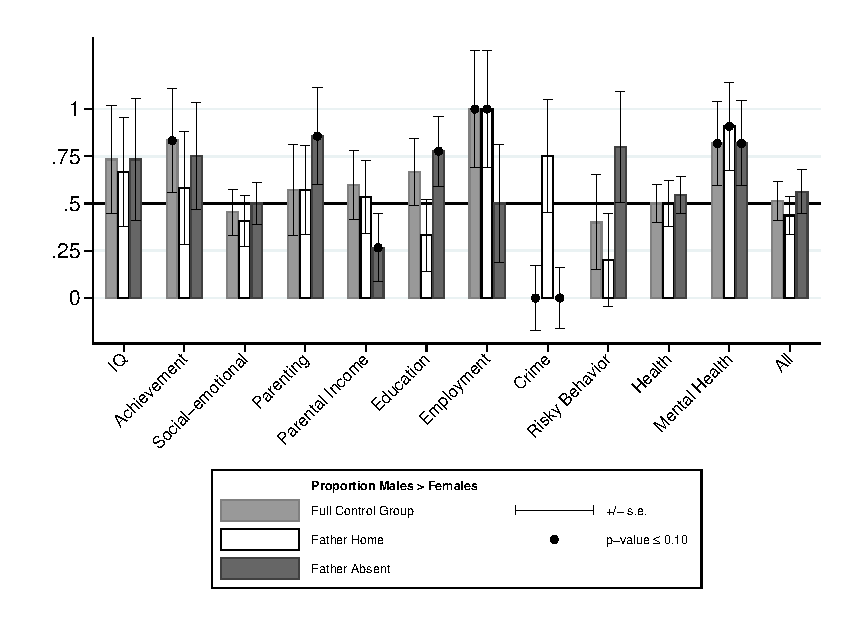
\includegraphics[width=\textwidth]{output/gendergaps-control-moderated-fhome}
	\end{subfigure}
	
\begin{subfigure}[h]{0.7\textwidth}
	\centering
	\caption{Treatment Group}
	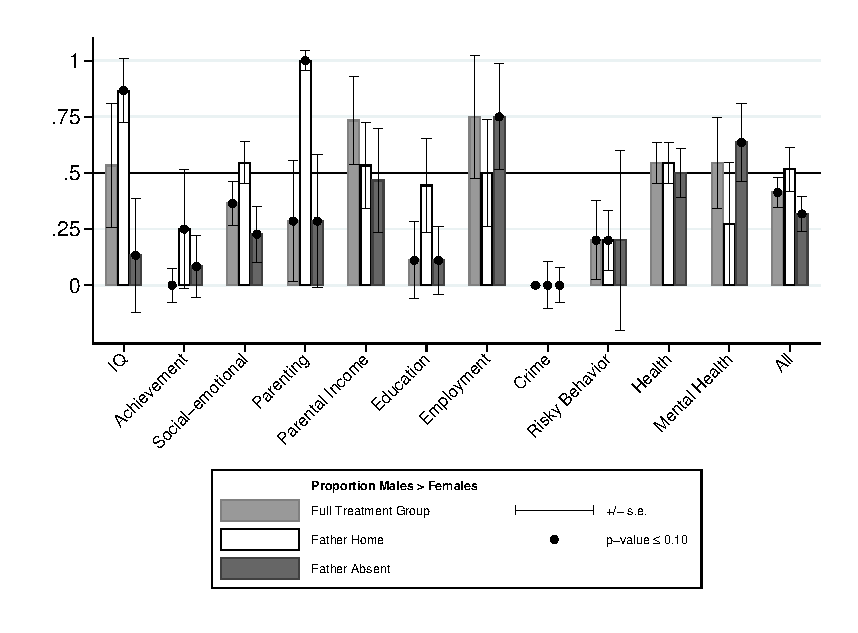
\includegraphics[width=\textwidth]{output/gendergaps-treatment-moderated-fhome}
	\end{subfigure}
\footnotesize \justify
Note: These plots show the proportion of outcomes, by outcome category, for which the males' mean is larger than the females' mean. The standard errors and the $p$-values are computed using 100 bootstraps. The $p$-values are one-sided and test the null hypothesis that the proportion of outcomes is greater than $\frac{1}{2}$ The crime outcomes are all coded so that a higher value indicates more criminal activity. All other outcome categories have higher values corresponding to socially desirable outcomes.
\end{figure}

Another measure of home environment maternal locus of control, which is measured when the subjects were 1.5 years old.\footnote{We define internal locus of control as scoring below the sample mean and an external locus of control as scoring at or above the sample mean. See \citet{Rotter_1966_PMGaA}.} An internal locus of control indicates feeling in control of future outcomes, including those related to child rearing. In contrast, an external locus of control indicates feeling that outside forces determine future outcomes (e.g. luck). Figure~\ref{fig:proportion-mlocus} shows the results from conditioning on this variable. In the control group, a higher maternal internal locus of control promotes better outcomes for males across all outcome categories except health. Another way to state this is that males are more negatively affected if their mothers have a lower external locus of control than are females. This is consistent with the analyses of \citet{Schore_2017_IMHJ} and \citet{golding2016psychology}. Although locus of control does not necessarily measure depression, this finding corresponds with \citet{Beeghly-etal_2017_IMHJ}, who find that increased maternal depression lead to worse outcomes for young males relative to females.

\begin{figure}[!htbp]
\centering
\caption{Proportion of Outcomes Males $>$ Females, by Outcome Category, Dividing by Maternal Locus of Control}
\label{fig:proportion-mlocus}
\begin{subfigure}[h]{0.7\textwidth}
	\centering
	\caption{Control Group}
	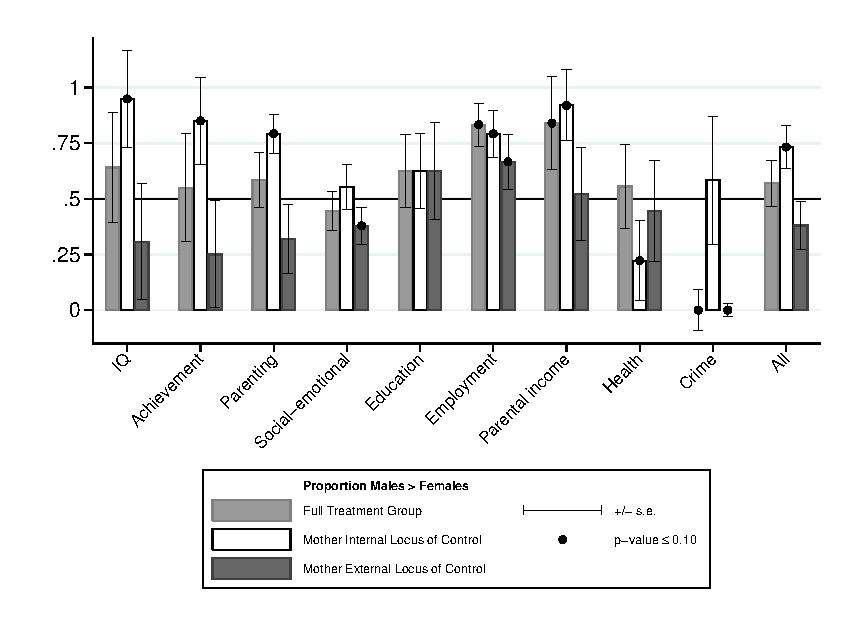
\includegraphics[width=\textwidth]{output/gendergaps-control-moderated-mlocus}
	\end{subfigure}
	
\begin{subfigure}[h]{0.7\textwidth}
	\centering
	\caption{Treatment Group}
	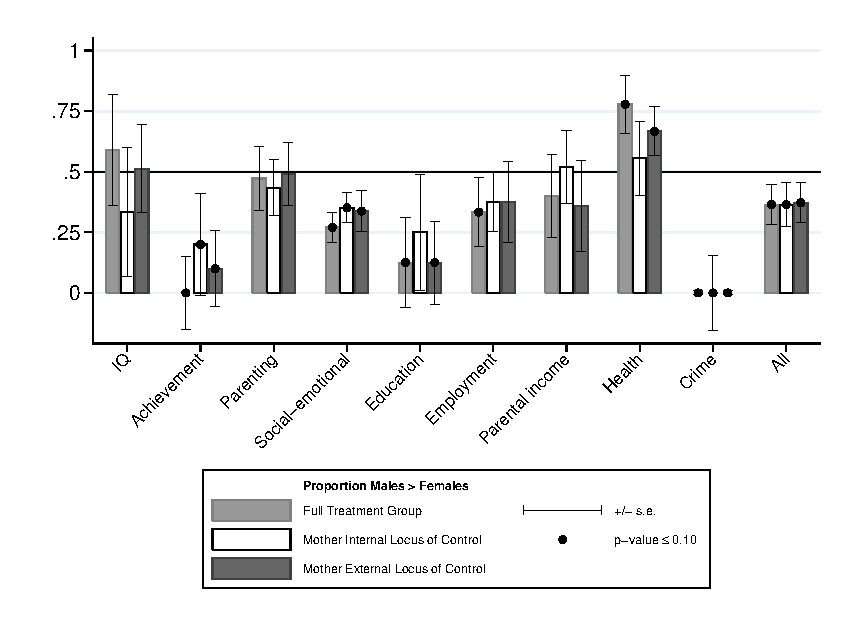
\includegraphics[width=\textwidth]{output/gendergaps-treatment-moderated-mlocus}
	\end{subfigure}
\footnotesize \justify
Note: These plots show the proportion of outcomes, by outcome category, for which the males' mean is larger than the females' mean. The standard errors and the $p$-values are computed using 100 bootstraps. The $p$-values are one-sided and test the null hypothesis that the proportion of outcomes is greater than $\frac{1}{2}$ The crime outcomes are all coded so that a higher value indicates more criminal activity. All other outcome categories have higher values corresponding to socially desirable outcomes.
\end{figure}

Maternal locus of control moderates the treatment outcomes differently. Regardless of locus of control males, do not do much better than their female counterparts. The exception is for health outcomes, in which the pattern of boys with mothers with external loci of control outperform those with mothers with internal loci of control. Treatment compensates for this form of disadvantage. Aggregating across outcomes, male outcomes are not much affected by the mother's locus of control if they attend ABC/CARE, while if they are in the control group, it does. This suggests an important compensating role of enriched early childhood programs.





\section{Conclusion}
\label{sec:conclusion}
This paper examines gender differences in the impacts of treatment of an influential early childhood program targeted to disadvantaged children. High-quality early childhood programs have positive effects on both boys and girls. 

We present results suggesting that lower-quality childcare arrangements are detrimental for boys relative to staying at home (if high-quality arrangements are not an option). We suggest that an explanation for this is the difference in baseline disadvantage between the boys and girls in the sample. The boys are more advantaged, with the more advantaged boys being more likely to stay at home. This explains why the effects are larger for males in comparison to alternative care than in comparison to staying at home. For girls, there is not an observed difference in advantage between the different counterfactual scenarios. The effects are still larger for girls in comparison to staying at home than in comparison to alternative care. This again reflects the disadvantage that the girls faced, although the difference between these estimates is smaller than the difference for boys.

Another aspect of these finding relates to literature on the biological, psychological, and social differences between boys and girls early in life. \citet{Schore_2017_IMHJ} and \citet{Eliot_Brain_2009_BOOK} provide helpful summaries of the current literature. Although there is some contention on the exact biological differences (see, e.g., \citet{Tan_Ma_Marwha_etal_2016_NI} and \citet{Eliot_2011_Sex-Diff_Neuron}), our findings are consistent with previous research that finds boys to be more vulnerable early in life than girls as a result of a confluence of biological, psychological, and social factors \citep{Beeghly-etal_2017_IMHJ}. The alternative programs available at the time of ABC/CARE were of lower quality. A more vulnerable child could be harmed in an environment that does not fully support his development.

Our analysis sounds a cautionary note about the value of early childcare programs. In the past decade, many politicians and pundits have warmly embraced early childhood programs as solutions for reducing inequality and promoting social mobility. Little attention has been paid to the quality of those programs. \cite{Garcia_Heckman_Leaf_etal_2017_Comp_CBA_Unpublished} show that they have a high economic rate of return. Even though we find that females benefit more than males overall, after weighing for the social benefits of reduced crime and improved health, education, and employment, the social return is higher for males than females. Although ABC/CARE had stronger effects on females, the monetary value of those effects are less than for males. 



\singlespacing
\bibliography{heckman}
\bibliographystyle{chicago}

\end{document}
